% =====================================================================================
% Rapport de projet de fin d'études — PC-FNO3D / ATOM Wind
% Ines Rouatbi — ESPRIT — Tukhnanutha (2026)
% Compilation : pdfLaTeX + BibTeX (compilateur par défaut d'Overleaf).
% Les éléments à compléter par l'autrice sont marqués \acompleter{...} (en rouge).
% =====================================================================================
\documentclass[12pt,a4paper,oneside]{report}

% ---------------------------------------------------------------- langue et polices
\usepackage[T1]{fontenc}
\usepackage[utf8]{inputenc}
\usepackage[french]{babel}
\usepackage{lmodern}
\usepackage{microtype}
\usepackage{csquotes}

% ---------------------------------------------------------------- mise en page
\usepackage[a4paper,top=2.5cm,bottom=2.5cm,left=2.8cm,right=2.3cm,headheight=15pt]{geometry}
\usepackage{setspace}
\onehalfspacing
\usepackage{fancyhdr}
\usepackage{titlesec}
\usepackage{xcolor}
\usepackage{graphicx}
\usepackage{float}
\usepackage{caption}
\usepackage{subcaption}
\usepackage{booktabs}
\usepackage{tabularx}
\usepackage{longtable}
\usepackage{multirow}
\usepackage{array}
\usepackage{enumitem}
\usepackage{amsmath,amssymb}
\usepackage{listings}
\usepackage{tikz}
\usetikzlibrary{arrows.meta,positioning,shapes.geometric,fit,backgrounds,calc}
\usepackage[numbers,sort&compress]{natbib}
\usepackage[hidelinks]{hyperref}
\usepackage{bookmark}

% ---------------------------------------------------------------- couleurs et styles
\definecolor{bleuespirt}{HTML}{2B6CB0}
\definecolor{grisdoux}{HTML}{4A5568}
\definecolor{fondcode}{HTML}{F7FAFC}
\newcommand{\acompleter}[1]{\textcolor{red}{[#1]}}
\newcommand{\code}[1]{\texttt{\small #1}}
\newcommand{\ms}{\,m/s}

\titleformat{\chapter}[display]
  {\normalfont\huge\bfseries\color{bleuespirt}}{\chaptertitlename\ \thechapter}{16pt}{\Huge}
\titlespacing*{\chapter}{0pt}{-20pt}{30pt}

\pagestyle{fancy}
\fancyhf{}
\fancyhead[L]{\small\color{grisdoux}\leftmark}
\fancyhead[R]{\small\color{grisdoux}PC-FNO3D / ATOM Wind}
\fancyfoot[C]{\thepage}
\renewcommand{\headrulewidth}{0.4pt}
\fancypagestyle{plain}{\fancyhf{}\fancyfoot[C]{\thepage}\renewcommand{\headrulewidth}{0pt}}

\lstset{basicstyle=\ttfamily\footnotesize, backgroundcolor=\color{fondcode}, frame=single,
        rulecolor=\color{grisdoux!40}, breaklines=true, columns=fullflexible,
        literate={é}{{\'e}}1 {è}{{\`e}}1 {à}{{\`a}}1 {ç}{{\c c}}1 {ê}{{\^e}}1 {ô}{{\^o}}1}

\captionsetup{font=small,labelfont=bf}
\setlist{itemsep=2pt,topsep=4pt}
\renewcommand{\arraystretch}{1.15}

% ---------------------------------------------------------------- informations
\newcommand{\titrerapport}{Reconstruction et prévision du champ de vent 3D\\[4pt]
  par un opérateur neuronal de Fourier contraint par la physique\\[4pt]
  \large(PC-FNO3D) et application web ATOM Wind}
\newcommand{\autrice}{Ines \textsc{Rouatbi}}

\begin{document}

% ---------------------------------------------------------------- pages liminaires
\pagenumbering{roman}
% ---------------------------------------------------------------- page de garde
\begin{titlepage}
\begin{center}
  {\large \textsc{République Tunisienne}}\\[2pt]
  {\small Ministère de l'Enseignement Supérieur et de la Recherche Scientifique}\\[14pt]
  % Logos : déposer les fichiers dans figures/ puis décommenter
  % \includegraphics[height=2cm]{figures/logo_esprit.png}\hfill
  % \includegraphics[height=2cm]{figures/logo_tukhnanutha.png}\\[10pt]
  {\Large \textbf{ESPRIT} --- École Supérieure Privée d'Ingénierie et de Technologies}\\[30pt]

  {\LARGE \textsc{Rapport de projet de fin d'études}}\\[8pt]
  {\large Présenté en vue de l'obtention du\\
  \textbf{Diplôme National d'Ingénieur} \acompleter{spécialité / option}}\\[26pt]

  \rule{\linewidth}{0.6pt}\\[10pt]
  {\Large \bfseries \color{bleuespirt} \titrerapport}\\[8pt]
  \rule{\linewidth}{0.6pt}\\[28pt]

  {\large Réalisé par : \textbf{\autrice}}\\[24pt]

  \begin{tabular}{ll}
    Encadrant académique : & \acompleter{Nom et prénom}\\[4pt]
    Encadrant professionnel : & \acompleter{Nom et prénom (Tukhnanutha)}\\
  \end{tabular}\\[30pt]

  {\large Organisme d'accueil : \textbf{Tukhnanutha}, Bizerte}\\[4pt]
  {Projet ANEO --- application ATOM Wind}\\[40pt]

  \vfill
  {\large Année universitaire 2025--2026}
\end{center}
\end{titlepage}

% ---------------------------------------------------------------- dédicace
\chapter*{Dédicace}
\addcontentsline{toc}{chapter}{Dédicace}
\begin{flushright}
\itshape
\acompleter{Texte de la dédicace, rédigé par l'autrice.}
\end{flushright}

% ---------------------------------------------------------------- remerciements
\chapter*{Remerciements}
\addcontentsline{toc}{chapter}{Remerciements}
\acompleter{Remerciements personnels : encadrant académique, encadrant professionnel et équipe de
Tukhnanutha, membres du jury, famille.}

% ---------------------------------------------------------------- résumé
\chapter*{Résumé}
\addcontentsline{toc}{chapter}{Résumé}
Ce projet de fin d'études, réalisé chez Tukhnanutha dans le cadre de l'écosystème ANEO, porte sur
la reconstruction du champ de vent tridimensionnel (composantes $u$, $v$, $w$) entre 25 et 1\,000\,m
d'altitude à partir de mesures de surface éparses. Nous avons conçu \emph{PC-FNO3D}, un opérateur
neuronal de Fourier 3D contraint par la physique : la perte combine l'erreur sur les données, la
régularité des gradients, la conservation anélastique de la masse $\nabla\cdot(\rho\vec{v})=0$ et
la condition au sol. Sur un jeu synthétique de 100 jours, le modèle de référence (v7) atteint
cinq des six objectifs mesurés (résidu de masse $2{,}6\cdot10^{-5}$, inférence en 91\,ms sur GPU,
robustesse à 25\,\% des capteurs) et divise par 7,5 à 9,8 l'erreur maximale des méthodes de
référence (profil logarithmique ou loi de puissance avec interpolation IDW ou krigeage). Le modèle a
ensuite été transposé au domaine réel du Grand Tunis (68\,$\times$\,56\,km) en apprenant une
correction du profil ERA5, avec une vérité générée forcée par ERA5 et une validation sur les
anémomètres réels et les radiosondages. Le modèle livré (v4) obtient une erreur globale de
0,38\,m/s, un résidu de masse de $1{,}05\cdot10^{-5}$ et une couverture calibrée de 88\,\% pour
l'intervalle à 80\,\%. Le tout est servi par une API sécurisée, un serveur MCP et l'application
web trilingue ATOM Wind (vue 3D, conseils agricoles de J0 à J+2, démonstration éolienne). Les
limites sont rapportées sans les masquer : le niveau le plus bas reste à 0,53\,m/s, et l'étude de
dimensionnement du réseau (OS6) montre que le modèle actuel ne tire aucun gain de capteurs ajoutés.

\noindent\textbf{Mots-clés :} champ de vent 3D, opérateur neuronal de Fourier, apprentissage
contraint par la physique, ERA5, GFS, quantification de l'incertitude, application web.

% ---------------------------------------------------------------- abstract
\chapter*{Abstract}
\addcontentsline{toc}{chapter}{Abstract}
\begin{otherlanguage}{english}
This final-year project, carried out at Tukhnanutha within the ANEO ecosystem, addresses the
reconstruction of the three-dimensional wind field ($u$, $v$, $w$) between 25 and 1,000\,m above
sea level from sparse surface measurements. We designed \emph{PC-FNO3D}, a physics-constrained 3D
Fourier neural operator whose loss combines the data error, a gradient term, anelastic mass
conservation $\nabla\cdot(\rho\vec{v})=0$ and the ground boundary condition. On a 100-day synthetic
dataset the reference model (v7) meets five of the six measured objectives (mass residual
$2.6\cdot10^{-5}$, 91\,ms GPU inference, robustness with 25\,\% of the sensors) and reduces the
worst-level error of the reference methods (log or power-law profile with IDW or kriging) by a
factor of 7.5 to 9.8. The model was then transferred to the real Greater Tunis domain
(68\,$\times$\,56\,km) by learning a correction of the ERA5 profile, with an ERA5-forced generated
truth and validation against real anemometers and radiosondes. The delivered model (v4) reaches a
global error of 0.38\,m/s, a mass residual of $1.05\cdot10^{-5}$ and a calibrated 88\,\% coverage
of the 80\,\% interval. It is served through a secured API, an MCP server and the trilingual ATOM
Wind web application (3D view, farming advice from day 0 to day 2, wind-energy demonstration).
Limits are reported as measured: the lowest level remains at 0.53\,m/s, and the network-sizing
study (OS6) shows that the current model gains nothing from additional sensors.

\noindent\textbf{Keywords:} 3D wind field, Fourier neural operator, physics-constrained learning,
ERA5, GFS, uncertainty quantification, web application.
\end{otherlanguage}


\tableofcontents
\listoffigures
\listoftables
\chapter*{Liste des abréviations}
\addcontentsline{toc}{chapter}{Liste des abréviations}
\begin{longtable}{@{}p{3cm}p{11.5cm}@{}}
\toprule
\textbf{Sigle} & \textbf{Signification}\\
\midrule
\endhead
ANEO & Réseau de capteurs environnementaux de l'écosystème Tukhnanutha\\
API & Interface de programmation (\emph{Application Programming Interface})\\
ATOM Wind & Application web de restitution du vent 3D (agriculture, éolien)\\
DEM & Modèle numérique de terrain (\emph{Digital Elevation Model})\\
DSO & Objectif de performance mesurable (critère d'acceptation du modèle)\\
EMA & Moyenne exponentielle des poids (\emph{Exponential Moving Average})\\
ERA5 & Cinquième réanalyse atmosphérique du CEPMMT (ECMWF)\\
FAO-56 & Méthode Penman-Monteith de la FAO pour l'évapotranspiration\\
FFT & Transformée de Fourier rapide\\
FNO & Opérateur neuronal de Fourier (\emph{Fourier Neural Operator})\\
GEFS & Ensemble de prévision global de la NOAA (31 membres)\\
GFS & Système de prévision global de la NOAA (\emph{Global Forecast System})\\
IDW & Pondération inverse à la distance (\emph{Inverse Distance Weighting})\\
IGRA & Archive mondiale des radiosondages (\emph{Integrated Global Radiosonde Archive})\\
INM & Institut National de la Météorologie (Tunisie)\\
MCP & Protocole de contexte de modèle (\emph{Model Context Protocol})\\
METAR & Message d'observation météorologique d'aérodrome\\
OMM & Organisation Météorologique Mondiale\\
OS & Objectif spécifique du cahier des charges\\
OSSE & Expérience de simulation de systèmes d'observation\\
PC-FNO3D & Opérateur neuronal de Fourier 3D contraint par la physique\\
RMSE & Racine de l'erreur quadratique moyenne\\
SYNOP & Message d'observation synoptique de station au sol\\
\bottomrule
\end{longtable}


% ---------------------------------------------------------------- corps
\cleardoublepage
\pagenumbering{arabic}
\chapter*{Introduction générale}
\addcontentsline{toc}{chapter}{Introduction générale}
\markboth{Introduction générale}{}

Le vent conditionne une grande partie des activités humaines exposées au climat : la réussite d'un
traitement phytosanitaire, la quantité d'eau perdue par une parcelle irriguée, la production d'une
éolienne, la sécurité d'un levage sur un chantier. Ces décisions se prennent à des hauteurs très
différentes --- 2 à 10\,m pour l'agriculture, 50 à 150\,m pour l'éolien --- et en des lieux où, le
plus souvent, aucun instrument ne mesure le vent. Les stations météorologiques sont rares, placées
près du sol, et les modèles numériques de prévision décrivent l'atmosphère sur des mailles de
plusieurs kilomètres qui lissent l'effet du relief et du littoral.

Tukhnanutha, holding technologique tunisienne, développe l'écosystème ANEO : un réseau de capteurs
environnementaux portés par des mâts multiservices, et des services numériques construits sur leurs
données. Ce projet de fin d'études répond à une question centrale de cet écosystème :
\emph{comment connaître le vent partout, à toutes les hauteurs utiles, à partir de mesures prises
en quelques points près du sol ?}

Nous y répondons par un modèle d'apprentissage profond contraint par la physique,
\textbf{PC-FNO3D}, un opérateur neuronal de Fourier tridimensionnel qui reconstruit en moins d'une
seconde les trois composantes du vent sur douze niveaux, de 25 à 1\,000\,m d'altitude. Le modèle
apprend sur des données dont il respecte la physique : la conservation de la masse et la condition
au sol font partie de sa fonction de perte. Il est ensuite transposé à un domaine réel, le Grand
Tunis, confronté aux mesures réelles des anémomètres et des radiosondages, et mis en service dans
une application web, \textbf{ATOM Wind}, destinée aux agriculteurs et aux exploitants éoliens.

Le travail s'est déroulé en plusieurs étapes qui structurent ce rapport :
\begin{itemize}
  \item le \textbf{chapitre~\ref{chap:contexte}} présente l'organisme d'accueil, le problème, les
        objectifs mesurables (DSO) fixés par le cahier des charges et la conduite du projet ;
  \item le \textbf{chapitre~\ref{chap:etat}} situe le travail par rapport aux méthodes classiques
        d'interpolation, aux modèles numériques de l'atmosphère et aux architectures d'apprentissage
        profond, dont celles que nous avons essayées puis abandonnées ;
  \item le \textbf{chapitre~\ref{chap:donnees}} décrit les données : le jeu synthétique ANEO, puis
        le domaine réel du Grand Tunis (relief, occupation du sol, ERA5, stations, radiosondages,
        prévisions GFS) ;
  \item le \textbf{chapitre~\ref{chap:modele}} détaille l'architecture PC-FNO3D, la perte physique,
        l'entraînement et la quantification de l'incertitude ;
  \item le \textbf{chapitre~\ref{chap:resultats}} rapporte les résultats, critère par critère, y
        compris les résultats négatifs et les décisions qui en ont découlé ;
  \item le \textbf{chapitre~\ref{chap:realisation}} présente la réalisation logicielle : paquet
        Python, API, serveur MCP, mise en service et application ATOM Wind ;
  \item la conclusion dresse le bilan et les perspectives.
\end{itemize}

Un principe a guidé tout le projet, celui de la preuve de concept de Nuthora Edu : \emph{un
résultat n'est retenu que s'il est mesuré face à des critères fixés à l'avance}. Cette exigence est
l'un des apports du travail : elle a permis d'écarter des pistes séduisantes mais fragiles
--- correction post-modèle, affinage sur les stations --- et de fonder chaque décision, y compris
les résultats négatifs, qui orientent directement la suite du projet.

\chapter{Contexte général du projet}
\label{chap:contexte}

\section{Organisme d'accueil}

\subsection{Tukhnanutha}
Tukhnanutha est une holding technologique tunisienne qui réunit un pôle de recherche appliquée et
des activités de services numériques. Le stage s'est déroulé au sein de son équipe de recherche et
développement, à Bizerte, sous l'encadrement de \acompleter{nom de l'encadrant professionnel}.
\acompleter{Compléter : date de création, effectif, secteurs d'activité, organigramme si souhaité.}

Le projet est porté par \textbf{Nuthora Edu}, le pôle de recherche appliquée et de formation de
Tukhnanutha, qui fournit son cadre de réalisation et sa démarche de preuve de concept
(section~\ref{sec:demarche}). Ses résultats intéressent directement plusieurs filiales du groupe,
en premier lieu \textbf{AGRO-IN}, consacrée à l'agriculture de précision, à laquelle s'adresse
l'espace agriculteur d'ATOM Wind.

\subsection{L'écosystème ANEO et le mât Porteur}
Les services de Tukhnanutha sont pensés pour être déployés sur le terrain au moyen d'une cellule
standardisée, le \emph{Porteur} : un mât multiservice qui associe mesure environnementale,
connectivité, énergie, supervision et stockage des données. Les mâts sont prévus en quatre
hauteurs (15, 20, 25 et 30\,m) et produisent leur propre énergie par une source hybride solaire et
éolienne. L'ensemble des capteurs portés par ces mâts forme le réseau \textbf{ANEO}.

Les capteurs ANEO mesurent près du sol, à la hauteur des mâts, et en des points séparés de
plusieurs centaines de mètres. Or les usages visés --- conseil agricole, estimation de la
production éolienne, choix des emplacements des mâts eux-mêmes --- demandent le vent partout et à
d'autres hauteurs. C'est l'objet de l'application \textbf{ATOM Wind}.

\section{Problématique}
Le problème se formule ainsi : \emph{à partir d'un instantané de mesures de surface éparses et
bruitées, reconstruire le champ de vent tridimensionnel $(u, v, w)$ sur tous les nœuds d'une grille
3D, du sol jusqu'à 1\,000\,m, en moins d'une seconde, en respectant les lois physiques et en
indiquant la confiance à accorder à chaque valeur.}

Trois difficultés rendent le problème délicat :
\begin{enumerate}
  \item \textbf{l'absence de vérité en altitude} : un réseau de surface ne mesure rien au-dessus de
        30\,m ; il faut donc une vérité d'apprentissage construite autrement (générateur physique,
        réanalyse) et la valider sur les rares mesures d'altitude existantes (radiosondages) ;
  \item \textbf{le relief et le littoral} : le terrain tunisien n'est pas plat ; une partie des
        niveaux bas est sous le relief, et la brise de mer domine le cycle diurne près des côtes ;
  \item \textbf{la contrainte de temps} : une reconstruction doit être servie en temps quasi réel,
        ce qui exclut un modèle numérique de méso-échelle relancé à chaque instant.
\end{enumerate}

\section{Objectifs}

\subsection{Objectifs spécifiques}
Le cahier des charges, révisé au fil du projet jusqu'à sa version 12, fixe les objectifs
spécifiques suivants :
\begin{itemize}
  \item \textbf{OS1 --- reconstruction spatiale} : apprendre le champ 3D à partir des mesures
        éparses ;
  \item \textbf{OS2 --- contraintes physiques} : imposer la conservation anélastique de la masse
        $\nabla\cdot(\rho\vec{v}) = 0$ et la condition au sol ;
  \item \textbf{OS6 --- plan de déploiement du réseau ANEO} : dire combien de capteurs installer
        et où, en simulant leur apport ;
  \item \textbf{OS7 --- prévision du vent 3D à +24 et +48\,h} : le même modèle nourri par la
        prévision GFS au lieu de la réanalyse ;
  \item \textbf{OS8 --- applications métier} : l'agriculture comme application principale
        (fenêtres de traitement et d'irrigation de J0 à J+2, besoin en eau FAO-56) et une
        démonstration éolienne entre 50 et 150\,m.
\end{itemize}

\subsection{Objectifs de performance mesurables (DSO)}
Le modèle est jugé sur des critères chiffrés, mesurés sur un jeu de test jamais utilisé pour le
régler (tableau~\ref{tab:dso}).

\begin{table}[H]
\centering
\caption{Objectifs de performance du modèle (DSO).}
\label{tab:dso}
\begin{tabularx}{\linewidth}{@{}lXl@{}}
\toprule
Code & Critère & Seuil\\
\midrule
DSO1 & Précision : RMSE de $u$ et $v$ à chaque niveau, et $R^2$ & $\le 0{,}5$\ms ; $R^2 \ge 0{,}95$\\
DSO2 & Conservation de la masse : résidu de $\nabla\cdot(\rho\vec v)$ normalisé & $\le 10^{-4}$\\
DSO3 & Finesse des détails : rapport de rugosité prédiction / vérité & dans $[0{,}9 ; 1{,}1]$\\
DSO4 & Rapidité : temps d'une carte 3D complète (GPU) & $< 1$\,s\\
DSO5 & Robustesse : RMSE avec 25\,\% des capteurs & $\le 0{,}7$\ms\\
DSO6 & Fiabilité : couverture de l'intervalle à 80\,\% et corrélation erreur--incertitude & $\approx 80\,\%$, corrélation $>0$\\
\bottomrule
\end{tabularx}
\end{table}

D'autres critères complètent ces DSO : la confrontation au réel (REEL1 : erreur aux stations
inférieure à celle d'ERA5 et d'une interpolation ; REEL2 : radiosondages), la prévision (PREV1 à
PREV3), les décisions agricoles (AGRI1, AGRI2), le réseau (NET1, NET2), les alertes (AN1), l'éolien
(EOL1, EOL2), les données (DE1 à DE3), l'API et le serveur MCP (API1, MCP1), l'historique (HIS1) et
l'expérience utilisateur (UX1, VIS1). Le bilan critère par critère est donné au
chapitre~\ref{chap:resultats}.

\section{Démarche méthodologique}
\label{sec:demarche}
La démarche suit celle que fixe le cahier des charges et combine trois niveaux complémentaires :
\textbf{TDSP} pour le cycle du projet, la \textbf{preuve de concept de Nuthora Edu} pour la
validation, et \textbf{Scrum} pour l'organisation du travail.

\subsection{Le cycle TDSP}
Le \emph{Team Data Science Process} (TDSP) de Microsoft organise un projet de science des données
en cinq étapes : compréhension du besoin, acquisition et compréhension des données, modélisation,
déploiement et acceptation par le client. Nous l'avons préféré à CRISP-DM parce que le projet ne
se limite pas à un modèle : il comprend une API, une application, un service temps réel et des
critères d'acceptation fixés avec l'entreprise, que TDSP couvre par des étapes dédiées
(déploiement, acceptation). Le tableau~\ref{tab:tdsp} relie chaque étape aux chapitres du rapport.

\begin{table}[H]
\centering
\caption{Étapes TDSP et chapitres du rapport.}
\label{tab:tdsp}
\begin{tabularx}{\linewidth}{@{}lXl@{}}
\toprule
Étape TDSP & Contenu & Chapitre\\
\midrule
Compréhension du besoin & Tukhnanutha, ANEO, ATOM Wind, AGRO-IN, problématique, objectifs, critères & 1\\
Données & Jeu synthétique, puis Grand Tunis : ERA5, stations INM, radiosondages, GFS & 3\\
Modélisation & État de l'art, PC-FNO3D, perte physique, entraînement, prévision (OS7) & 2 et 4\\
Déploiement & Paquet, API, temps réel, application, espaces agriculteur et éolien & 6\\
Acceptation & Résultats face aux critères, bilan de conformité, décisions & 5 et conclusion\\
\bottomrule
\end{tabularx}
\end{table}

TDSP n'est pas une suite linéaire : c'est un cycle qui prévoit les retours vers une étape
antérieure quand une mesure le justifie. Le projet en a tiré pleinement parti
(figure~\ref{fig:tdsp}) : chaque retour a été déclenché par un résultat mesuré et a conduit à un
modèle meilleur ou à une décision mieux fondée.

\begin{figure}[H]
\centering
\begin{tikzpicture}[
  etape/.style={draw, rounded corners=4pt, align=center, font=\footnotesize\bfseries,
                text width=2.3cm, minimum height=1.1cm, fill=bleuespirt!10},
  cycle/.style={-{Stealth[length=2.5mm]}, line width=1.2pt, bleuespirt},
  retour/.style={-{Stealth[length=2mm]}, thick, dashed, orange!80!black},
  note/.style={font=\scriptsize, align=center, text=orange!60!black, inner sep=1pt}]
  \node[etape] (b) at (0, 0)    {Besoin};
  \node[etape] (d) at (3.0, 0) {Données};
  \node[etape] (m) at (6.0, 0)  {Modélisation};
  \node[etape] (p) at (9.0, 0) {Déploiement};
  \node[etape] (a) at (12.0, 0) {Acceptation};
  \draw[cycle] (b) -- (d);
  \draw[cycle] (d) -- (m);
  \draw[cycle] (m) -- (p);
  \draw[cycle] (p) -- (a);
  % retours au-dessus
  \draw[retour] (m.north) to[out=110, in=70, looseness=1.2] node[note, above]
    {2D $\rightarrow$ 3D\\synthétique $\rightarrow$ réel} (d.north);
  \draw[retour] (p.north) to[out=110, in=70, looseness=1.2] node[note, above]
    {temps réel\\ERA5 $\rightarrow$ GFS} (m.north);
  % retours au-dessous
  \draw[retour] (a.south) to[out=-110, in=-70, looseness=0.9] node[note, below]
    {v1 $\rightarrow$ v2 ; v3 écartée $\rightarrow$ v4\\M1 non retenue} (m.south);
  \draw[retour] (a.south east) to[out=-70, in=-110, looseness=0.75] node[note, below]
    {OS6 : vers un modèle qui exploite des capteurs denses} (b.south west);
\end{tikzpicture}
\caption{Le cycle TDSP du projet et ses itérations (flèches en pointillé).}
\label{fig:tdsp}
\end{figure}

\subsection{La preuve de concept selon Nuthora Edu}
La validation suit la démarche de preuve de concept de Nuthora Edu : une hypothèse testable, des
critères d'acceptation fixés \emph{avant} les essais (DSO, PREV, AGRI, EOL), une comparaison à une
méthode de référence (interpolation IDW et krigeage, ERA5, GFS brut, persistance), puis une
décision explicite. Cette discipline a été appliquée à chaque choix important : la correction M1,
l'affinage sur les stations (v3) et la livraison de la v4 ont chacun été jugés par une règle écrite
avant la lecture du test, ce qui garantit que les résultats rapportés ne sont pas le fruit d'un
réglage a posteriori.

\subsection{L'organisation Scrum}
Le travail a été organisé en itérations courtes selon Scrum : un backlog de fonctionnalités et
d'expériences issues du cahier des charges, des itérations dont chacune se termine par un
livrable mesuré, et une revue avec l'encadrant professionnel qui valide la décision et l'ordre des
prochaines tâches. La seconde moitié du projet a été découpée en lots de clôture (M0 à M8), chacun
avec son critère d'acceptation et sa revue. \acompleter{Préciser l'outil de suivi utilisé (Trello,
Jira, tableau partagé) et la cadence des revues.}

\subsection{Pratiques d'ingénierie}
\begin{itemize}
  \item \textbf{séparation stricte validation / test} : tout ce qui se règle (poids de la perte,
        choix du modèle, calibration de l'incertitude, seuils d'alerte) se règle sur la validation ;
        le code refuse un fichier de réglage marqué \enquote{test} ;
  \item \textbf{MLOps} : entraînement reproductible et reprenable, résultats de chaque expérience
        archivés dans un dossier nommé, empreintes SHA-256 des poids et des statistiques de
        normalisation dans chaque export, fiches du modèle et des données (\emph{model card},
        \emph{data card}) ;
  \item \textbf{qualité logicielle} : dépôt Git privé, une branche par lot, 435 fonctions de test
        réparties dans 42 fichiers, intégration continue ;
  \item \textbf{conception} : diagrammes UML (cas d'utilisation, classes, séquences) et
        architecture décrite à plusieurs niveaux de détail ;
  \item \textbf{calcul sur GPU à la demande} : entraînements et évaluations sur Google Colab
        (A100 et L4), données et résultats sur Google Drive, reprise automatique après coupure.
\end{itemize}

\section{Planification}

\subsection{Planification initiale}
La planification initiale prévoyait neuf tâches de mars à septembre 2026
(figure~\ref{fig:gantt}) : compréhension de la dynamique du vent, préparation des données,
conception du modèle, contraintes physiques, entraînement, reconstruction 3D, évaluation,
visualisation, déploiement.

\begin{figure}[H]
  \centering
  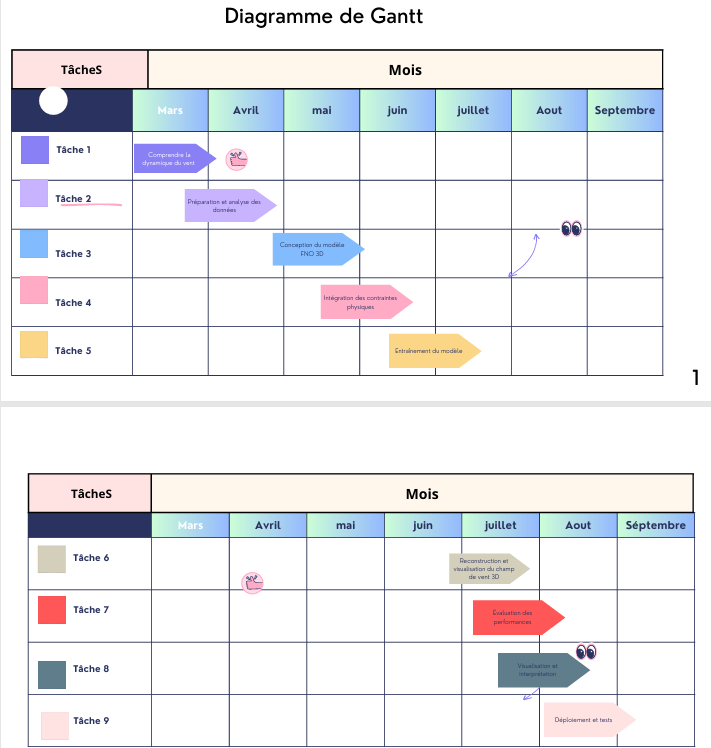
\includegraphics[width=0.82\linewidth]{figures/gantt_prevu.png}
  \caption{Diagramme de Gantt prévisionnel (mars--septembre 2026).}
  \label{fig:gantt}
\end{figure}

\subsection{Évolution du plan au fil des résultats}
Conformément au cycle TDSP, le plan a été adapté au fil des résultats
(tableau~\ref{tab:deroulement}). Une phase d'exploration large, qui a comparé six familles
d'architectures, a permis de converger vers un opérateur 3D unique ; la seconde moitié du projet,
organisée en lots courts terminés chacun par une mesure et une décision, a ensuite enchaîné le
modèle de référence, le passage aux données réelles, la mise en service et les études OS6 et OS7,
au-delà du périmètre prévu initialement.

\begin{table}[H]
\centering
\caption{Évolution du projet.}
\label{tab:deroulement}
\begin{tabularx}{\linewidth}{@{}p{3.2cm}X@{}}
\toprule
Période & Travaux\\
\midrule
mars -- juin 2026 & Étude de la dynamique du vent, génération des premières données ANEO, analyse exploratoire\\
juin -- sept. 2026 & Exploration de six familles d'architectures 2D (FNO 2D, U-Net/FNO, GNN, DeepONet, ResNet, ViT) ; extrapolation verticale séparée\\
fin sept. 2026 & Jeu synthétique 3D (\code{aneo\_dataset\_3d\_v2}, 12 niveaux) ; passage à un opérateur 3D supervisé directement\\
début oct. 2026 & Modèle de référence \textbf{v7} (140 époques, A100) ; portage du notebook en paquet Python testé\\
11 -- 16 oct. 2026 & Lots de clôture M0 à M8 : reproductibilité, fiabilité, contrat de données, alertes, éolien, publication, API, preuves ; tentative bornée M1 sur DSO1\\
21 -- 24 oct. 2026 & Domaine réel du Grand Tunis : générateur forcé par ERA5, modèles v1, v2, v2 prolongée, v3 (affinage sur stations, écarté), \textbf{v4} (livrée)\\
25 -- 31 oct. 2026 & Application ATOM Wind, temps réel GFS, cahier des charges v12, OS6 (plan du réseau)\\
nov. 2026 & OS7 (prévision +24/+48\,h) \acompleter{résultats à reporter}, rédaction\\
\bottomrule
\end{tabularx}
\end{table}


\chapter{État de l'art}
\label{chap:etat}

\section{Le vent dans la couche limite atmosphérique}

\subsection{Profil vertical}
Près du sol, le vent est freiné par la rugosité de la surface. Dans la couche de surface et en
atmosphère neutre, la vitesse croît avec la hauteur selon le profil logarithmique
\begin{equation}
  U(z) = \frac{u_*}{\kappa}\,\ln\!\left(\frac{z}{z_0}\right),
\end{equation}
où $u_*$ est la vitesse de frottement, $\kappa \approx 0{,}4$ la constante de von Kármán et $z_0$
la longueur de rugosité \citep{stull1988}. En pratique on utilise aussi la loi de puissance
$U(z) = U(z_r)\,(z/z_r)^{\alpha}$, dont l'exposant $\alpha$ dépend de la stabilité et du terrain.
Ces lois décrivent mal les situations stables, le relief et les transitions entre la couche limite
et l'atmosphère libre, où le vent tend vers le vent géostrophique imposé par le gradient de
pression à grande échelle.

\subsection{Phénomènes locaux}
Sur le littoral tunisien, la \textbf{brise de mer} --- un vent de mer vers terre dans la journée,
dû au contraste de température terre--mer --- impose un cycle diurne marqué de la direction du vent.
Le relief canalise et accélère l'écoulement, crée des zones abritées et des ascendances. Ces
phénomènes ont des échelles de quelques kilomètres, plus fines que les mailles des modèles globaux.

\subsection{Conservation de la masse}
Pour les mouvements de la couche limite, l'approximation anélastique \citep{ogura1962} remplace
l'équation de continuité complète par
\begin{equation}
  \nabla\cdot(\rho_0\,\vec v) = \frac{\partial(\rho_0 u)}{\partial x}
  + \frac{\partial(\rho_0 v)}{\partial y} + \frac{\partial(\rho_0 w)}{\partial z} = 0,
  \label{eq:anelastique}
\end{equation}
où $\rho_0(z)$ est la densité de référence. Cette relation lie la composante verticale $w$ à la
divergence horizontale, et sert à la fois de contrainte d'apprentissage et de critère (DSO2).

\section{Méthodes classiques de reconstruction}

\subsection{Interpolation spatiale}
La pondération inverse à la distance (IDW) \citep{shepard1968} estime la valeur en un point par
une moyenne des mesures pondérée par l'inverse d'une puissance de la distance. Le krigeage
\citep{cressie1993} choisit les poids qui minimisent la variance d'erreur sous un modèle de
covariance (variogramme) ajusté aux données. Combinées à une loi verticale (profil logarithmique
ou loi de puissance), ces méthodes forment les références auxquelles le modèle est comparé
(chapitre~\ref{chap:resultats}). Elles ignorent la physique de l'écoulement et le relief entre les
points de mesure.

\subsection{Modèles numériques et réanalyses}
Les modèles de méso-échelle comme WRF \citep{skamarock2019} résolvent les équations primitives sur
une grille fine et décrivent correctement brise et relief, mais une simulation coûte des heures de
calcul. Les \textbf{réanalyses} combinent un modèle et toutes les observations disponibles :
ERA5 \citep{hersbach2020} fournit l'état de l'atmosphère heure par heure depuis 1940 sur une
grille de 0,25° (environ 25\,km), et ERA5-Land \citep{munozsabater2021} la surface à 0,1°. ERA5
n'est disponible qu'avec environ cinq jours de retard. En temps réel et en prévision, on dispose
des modèles opérationnels, comme le GFS de la NOAA (0,25°, échéances horaires puis triho\-raires) et
son ensemble GEFS.

\section{Apprentissage profond pour les champs physiques}

\subsection{Réseaux convolutifs et graphes}
Les réseaux convolutifs, en particulier l'U-Net \citep{ronneberger2015}, sont devenus la référence
pour les problèmes de type image-à-image, dont la descente d'échelle des champs météorologiques.
Les réseaux de neurones sur graphes traitent naturellement des capteurs irrégulièrement répartis ;
GraphCast \citep{lam2023} les a portés à la prévision météorologique globale.

\subsection{Opérateurs neuronaux}
Un opérateur neuronal apprend une application entre espaces de fonctions plutôt qu'entre vecteurs
de taille fixe. DeepONet \citep{lu2021} sépare une branche qui encode la fonction d'entrée et un
tronc qui encode la position de sortie. L'\textbf{opérateur neuronal de Fourier} (FNO)
\citep{li2021fno} paramètre le noyau d'intégration directement dans l'espace de Fourier :
\begin{equation}
  (\mathcal{K}v)(x) = \mathcal{F}^{-1}\!\big(R_\phi \cdot \mathcal{F}(v)\big)(x),
\end{equation}
où $R_\phi$ est une matrice de poids complexes appliquée aux $k_{\max}$ premiers modes. Chaque
couche voit tout le domaine (champ récepteur global), le coût est celui d'une FFT, et le modèle
apprend des solutions d'équations aux dérivées partielles avec une précision qui a ouvert la voie à
FourCastNet \citep{pathak2022} en prévision globale.

\subsection{Apprentissage contraint par la physique}
Les réseaux informés par la physique (PINN) \citep{raissi2019} ajoutent à la perte le résidu des
équations du problème. Le PINO \citep{li2024pino} combine opérateur neuronal et perte physique.
Dans notre cas, la physique entre de deux façons : par la perte (résidu de masse discret,
condition au sol) et par la construction (composante $w$ recalculée par continuité dans le modèle
livré, section~\ref{sec:wcont}).

\section{Architectures explorées dans le projet}
La première moitié du projet a exploré six familles d'architectures 2D, chacune reconstruisant le
champ horizontal à hauteur de capteur, l'extrapolation verticale étant faite séparément par des
lois de profil (tableau~\ref{tab:archi}).

\begin{table}[H]
\centering
\caption{Architectures explorées puis abandonnées.}
\label{tab:archi}
\begin{tabularx}{\linewidth}{@{}lX@{}}
\toprule
Architecture & Raison de l'abandon\\
\midrule
FNO 2D (trois variantes) & Champ horizontal seulement ; perte de masse 2D sans le terme $\partial(\rho w)/\partial z$ ni correction du relief\\
U-Net / FNO & Même limite 2D ; pas de gain mesuré sur le FNO 2D\\
GNN & Entraînement non abouti (aucun point de contrôle exploitable)\\
DeepONet & Entraîné, mais sortie 2D et coût d'évaluation point par point\\
ResNet, ViT & Références sans structure physique ; ViT non abouti\\
\bottomrule
\end{tabularx}
\end{table}

Deux constats ont décidé du changement de direction. D'une part, la contrainte de masse calculée
en 2D omettait le terme vertical de l'équation~\eqref{eq:anelastique} et traitait un pas
horizontal sur un terrain en pente comme un pas à altitude constante : le critère DSO2 n'était pas
mesuré sur la bonne équation. D'autre part, le générateur de données a été étendu pour produire des
cibles 3D sur douze niveaux : un opérateur supervisé directement en 3D devenait possible. Nous
avons donc convergé sur une seule architecture, le FNO 3D contraint par la physique, décrit au
chapitre~\ref{chap:modele}.

\section{Positionnement}
PC-FNO3D se situe entre les méthodes d'interpolation, rapides mais aveugles à la physique, et les
modèles numériques, physiques mais coûteux. Il reprend l'efficacité du FNO (une passe en moins
d'une seconde sur GPU), y ajoute la physique de la couche limite par la perte et par la
construction de $w$, et, dans sa version réelle, apprend une \emph{correction} du profil ERA5 plutôt
que le champ entier : la grande échelle vient de la réanalyse (ou de la prévision GFS), le réseau
apporte le relief, le littoral et les mesures locales.

\chapter{Données}
\label{chap:donnees}

Le projet a utilisé deux familles de données : un jeu \textbf{synthétique} produit par un
générateur physique, qui a servi à mettre au point la méthode, puis le domaine \textbf{réel} du
Grand Tunis, construit à partir de données ouvertes. Dans les deux cas, la vérité en altitude est
\emph{générée} : aucune mesure ne couvre le volume 3D. Nous parlons donc de \enquote{vérité
d'apprentissage} et réservons le mot \enquote{mesure} aux observations réelles.

\section{Le jeu synthétique ANEO}

\subsection{Génération}
Le générateur de l'écosystème ANEO produit, pour chaque instant, l'état de surface sur une grille
fine et le champ 3D correspondant, de façon cohérente avec la dynamique de la couche limite (vent
géostrophique, cisaillement, brise, relief). Le jeu \code{aneo\_dataset\_3d\_v2}, généré le
28 septembre 2026, est décrit au tableau~\ref{tab:synth}.

\begin{table}[H]
\centering
\caption{Caractéristiques du jeu synthétique \code{aneo\_dataset\_3d\_v2}.}
\label{tab:synth}
\begin{tabularx}{\linewidth}{@{}lX@{}}
\toprule
Élément & Valeur\\
\midrule
Durée & 100 jours, 1\,000 instants (environ 35\,Go)\\
Domaine & 50\,$\times$\,25\,km, relief jusqu'à 677\,m\\
Grille de surface & 1\,000\,$\times$\,500 points au pas de 50\,m\\
Nœuds 3D (cible) & 500\,$\times$\,250 au pas de 100\,m, 12 niveaux au-dessus du niveau de la mer : 25, 50, 75, 100, 150, 200, 300, 400, 500, 650, 800 et 1\,000\,m\\
Nœuds valides & 849\,184 au-dessus du relief (environ 1,5 million de nœuds de grille par instant)\\
Entrées de surface & vent $u$, $v$, $w$, température, densité, humidité relative, pression, et indicateur de mesure \code{mask\_i\_obs}\\
Cibles & $u$, $v$, $w$ et $\rho$ aux nœuds 3D\\
Découpage & par jour entier, 70 / 15 / 15\,\% (entraînement / validation / test)\\
Test & 166 instants : 120 synoptiques (heure pleine, multiple de 3\,h) et 46 d'épisodes rapides (rafales, front, brise), rapportés à part\\
\bottomrule
\end{tabularx}
\end{table}

Le contrôle qualité du générateur passe toutes ses vérifications (résidu de masse maximal
$6{,}4\cdot10^{-12}$, corrélations spatiales et temporelles, équilibre hydrostatique) sauf
l'équilibre des secteurs de direction (0,095 pour un seuil de 0,10), un défaut mineur non bloquant.

\subsection{Limites du jeu synthétique}
La couche de surface du générateur est quasi continue : environ 62\,000 points de mesure visibles
à 50\,\%, alors qu'un réseau ANEO réel compte un capteur tous les 500\,m à 1\,km. Le modèle entraîné
sur ce jeu voit donc beaucoup plus d'information qu'il n'en aura en production. Par ailleurs, la
position géographique du domaine synthétique est supposée : aucune mesure réelle ne peut y être
placée. Ces deux limites ont motivé le passage au domaine réel.

\subsection{Contrat de données}
Les fichiers de mesures ANEO suivent un contrat de données (critère DE1) : colonnes et types
attendus, plages physiques, règles de cohérence et indicateurs de qualité (valeurs hors plage,
figées, absentes, interpolées). Chaque fichier reçoit un verdict \enquote{conforme},
\enquote{quarantaine} ou \enquote{rejet} accompagné d'un rapport ; un fichier en quarantaine est
tout de même reconstruit, les stations signalées étant masquées.

\section{Le domaine réel du Grand Tunis}

\subsection{Grille et surface}
Le domaine réel couvre 68\,$\times$\,56\,km, de 36,395 à 36,900°\,N et de 10,04 à 10,80°\,E. Le
relief provient du modèle numérique de terrain Copernicus, et la rugosité $z_0$ de l'occupation du
sol ESA WorldCover \citep{zanaga2021}, sur une grille de surface au pas de 50\,m. Les nœuds 3D sont
au pas de 100\,m sur les douze niveaux du jeu synthétique : une grille de
12\,$\times$\,560\,$\times$\,680, dont 3\,469\,007 nœuds valides sur 4\,569\,600. La part du domaine
au-dessus du relief va de 26\,\% à 25\,m à 100\,\% à partir de 650\,m.

\subsection{Forçage ERA5 et vérité générée}
La vérité d'apprentissage est produite par le générateur \emph{forcé par ERA5} : pour chaque
instant, la grande échelle (vent géostrophique, cisaillement et rotation avec l'altitude, stabilité,
contraste de température terre--mer) est calculée à partir d'ERA5 sur les mailles qui couvrent le
domaine, puis le générateur y ajoute la brise de mer et l'effet du relief. La grande échelle est
recalée sur ERA5 maille par maille à la même hauteur au-dessus du sol, et $w$ est obtenu par
continuité. Deux portes de contrôle ont précédé la génération complète :
\begin{itemize}
  \item un jour d'hiver test : conservation de la masse exacte, moyenne du domaine égale à ERA5 à
        chaque niveau, erreur aux trois stations au plus égale à celle d'ERA5 ;
  \item le cycle diurne de la direction en été à Tunis-Carthage et Nabeul (brise de mer), validé
        visuellement avant la génération.
\end{itemize}

\textbf{Règle d'usage des stations} : les mesures des stations n'entrent jamais dans la vérité
d'apprentissage. Elles servent d'entrée au modèle et de référence de validation, ce qui garde la
validation sur le réel indépendante.

\subsection{Mesures réelles}
\begin{table}[H]
\centering
\caption{Sources de données réelles.}
\label{tab:sources}
\begin{tabularx}{\linewidth}{@{}lXl@{}}
\toprule
Source & Contenu & Usage\\
\midrule
METAR DTTA & Tunis-Carthage, vent à 10\,m, horaire & entrée, validation\\
SYNOP 60729, 60728 & Zaghouan et Nabeul (INM, via NOAA ISD), vent à 10\,m, triho\-raire & entrée, validation\\
IGRA TSM00060715 & Radiosondages de Tunis-Carthage & validation en altitude\\
ERA5, ERA5-Land & Réanalyse horaire, 0,25° et 0,1° & forçage, entrée du modèle\\
GFS & Prévision NOAA 0,25° (temps réel et archive AWS) & temps réel, OS7\\
GEFS & Ensemble de 31 membres & prévision probabiliste\\
Copernicus DEM, WorldCover & Relief et occupation du sol & grille, rugosité\\
\bottomrule
\end{tabularx}
\end{table}

Les séries ont été nettoyées : à Nabeul, l'anémomètre est resté à zéro en juin, juillet et
septembre 2021 (mois masqués), et les années 2023--2024, où la station est abritée, sont exclues.

\subsection{Découpage temporel}
Le découpage est temporel et fixé une fois pour toutes : le \textbf{test} couvre janvier--mars et
juillet--août 2022 (hiver et été), la \textbf{validation} janvier--février et juillet 2021, et
l'\textbf{entraînement} le reste de 2021 à 2025, avec une marge de sept jours autour des blocs de
validation et de test. Le cache du modèle compte 700 instants d'entraînement, 120 de validation et
180 de test (environ 49\,Mo par instant).

\subsection{Entrée de production}
Avec trois stations seulement dans le domaine, la couche de surface dense du jeu synthétique n'a
pas d'équivalent réel. L'entrée de production est donc formée de \textbf{pseudo-capteurs ERA5} à
10\,m tous les 2,5\,km, des \textbf{cellules des stations} réelles, des \textbf{sept scalaires de
forçage} de l'instant et du \textbf{profil ERA5} interpolé à chaque nœud. En temps réel et en
prévision, la prévision GFS remplace ERA5, avec les mêmes formules et les mêmes mailles.

\chapter{Le modèle PC-FNO3D}
\label{chap:modele}

\section{Formulation}
Pour un instant $t$, le modèle reçoit un tenseur d'entrée $X_t \in \mathbb{R}^{C\times n_z\times
n_y\times n_x}$ qui porte les mesures de surface recopiées sur la colonne, le relief, la géométrie
des niveaux et des caractéristiques temporelles et physiques, et produit
$\hat Y_t \in \mathbb{R}^{3\times n_z\times n_y\times n_x}$, les composantes $(u, v, w)$ en chaque
nœud. Les nœuds sous le relief sont exclus de toutes les pertes et de toutes les métriques par un
masque de validité. Le modèle est un \emph{opérateur} : il apprend l'application qui associe un
état de surface à un champ 3D, et non une interpolation point par point.

\section{Architecture}
L'architecture (figure~\ref{fig:archi}) suit le schéma du FNO \citep{li2021fno} étendu à trois
dimensions :
\begin{enumerate}
  \item une couche de \textbf{relèvement} $P$ (convolution $1\times1\times1$) porte les $C$ canaux
        d'entrée à une largeur de 48 ;
  \item quatre \textbf{couches de Fourier} : chacune applique une convolution spectrale sur les
        modes de plus basse fréquence ($6\times32\times32$ selon $z$, $y$, $x$), ajoute une branche
        convolutive locale, puis une activation GELU ; un rembourrage $(4, 8, 8)$ évite les effets
        de périodicité de la FFT ;
  \item une \textbf{tête de projection} $Q$ (couche cachée de 128) produit $u$, $v$ et $w$.
\end{enumerate}
Le modèle compte 453 millions de paramètres, dont l'essentiel dans les poids spectraux complexes.
Le calcul se fait en bfloat16 sur GPU, sauf deux îlots en float32 volontaires --- la FFT et la tête
de projection --- : sans eux, le bruit d'arrondi passe dans les différences centrées du résidu de
masse et l'empêche de descendre sous le seuil du DSO2.

\begin{figure}[H]
\centering
\begin{tikzpicture}[
  bloc/.style={draw, rounded corners=3pt, minimum height=1.0cm, minimum width=1.6cm,
               align=center, font=\small, fill=bleuespirt!10},
  four/.style={bloc, fill=orange!15, minimum width=1.9cm},
  fl/.style={-{Stealth[length=2.5mm]}, thick}]
  \node[bloc, fill=gray!10] (x) {Entrée $X_t$\\ \footnotesize $C\times12\times n_y\times n_x$};
  \node[bloc, right=0.55cm of x] (p) {Relèvement\\$P$};
  \node[four, right=0.55cm of p] (f1) {Couche\\de Fourier};
  \node[font=\large, right=0.25cm of f1] (dots) {$\cdots$};
  \node[four, right=0.25cm of dots] (f4) {Couche\\de Fourier};
  \node[bloc, right=0.55cm of f4] (q) {Projection\\$Q$};
  \node[bloc, fill=gray!10, right=0.55cm of q] (y) {$u, v, w$};
  \draw[fl] (x) -- (p); \draw[fl] (p) -- (f1); \draw[fl] (f1) -- (dots);
  \draw[fl] (dots) -- (f4); \draw[fl] (f4) -- (q); \draw[fl] (q) -- (y);
  \node[below=1.2cm of f1, draw, dashed, rounded corners, align=center, font=\footnotesize,
        text width=8.6cm] (det)
    {$v_{\ell+1} = \sigma\!\left(\mathcal{F}^{-1}\big(R_\ell\cdot\mathcal{F}(v_\ell)\big)
      + W_\ell\, v_\ell\right)$\\[2pt] FFT 3D (float32), $R_\ell$ sur $6\times32\times32$ modes,
      $W_\ell$ branche locale, $\sigma$ = GELU};
  \draw[dashed, gray] (f1.south) -- (det.north);
  \node[below=0.35cm of y, font=\footnotesize, align=center, text=grisdoux]
    {réel : $u, v$ = ERA5\\+ correction ;\\$w$ par continuité};
\end{tikzpicture}
\caption{Architecture de PC-FNO3D.}
\label{fig:archi}
\end{figure}

\section{Canaux d'entrée}
Le modèle de référence synthétique (v7) reçoit 25 canaux :
\begin{itemize}
  \item les 7 mesures de surface normalisées ($u$, $v$, $w$, température, densité, humidité,
        pression) et une carte de disponibilité, qui vaut 1 là où un capteur est visible ;
  \item 6 canaux de relief : altitude du terrain, logarithme de la rugosité, pente, sinus et
        cosinus de l'orientation, hauteur du capteur ;
  \item 3 canaux de géométrie par niveau (altitude du niveau, hauteur au-dessus du sol, validité) ;
  \item 8 canaux temporels et physiques : heure et jour de l'année, et un vent géostrophique et un
        vent thermique ajustés par moindres carrés sur les capteurs visibles de l'instant.
\end{itemize}
Le modèle réel en ajoute 9, placés en dernier : les 7 scalaires de forçage ERA5 (vent géostrophique
$u_g$, $v_g$, cisaillement, rotation, stabilité, contraste terre--mer) et le vent ERA5 $u$, $v$
interpolé à chaque nœud, soit 34 canaux.

\section{Sortie résiduelle sur ERA5}
Le premier modèle réel (v1), entraîné à prédire le champ entier, plafonnait à $R^2 = 0{,}78$ pour
$u$ en validation, alors que le profil ERA5 interpolé aux nœuds, seul, atteint 0,95 : il manquait à
l'entrée l'information de grande échelle. Le modèle v2 apprend donc une \textbf{correction} :
\begin{equation}
  \hat u = u_{\mathrm{ERA5}} + \Delta u_\theta(X), \qquad
  \hat v = v_{\mathrm{ERA5}} + \Delta v_\theta(X).
\end{equation}
Lors de l'initialisation depuis un modèle à 25 canaux, les colonnes de la couche de relèvement
correspondant aux nouveaux canaux et les lignes $u$, $v$ de la dernière projection sont mises à
zéro : l'entraînement part exactement d'ERA5 et n'apprend que l'écart.

\section{Fonction de perte}
La perte combine un terme de données et des termes physiques :
\begin{equation}
  \mathcal{L} = \mathcal{L}_{\mathrm{data}} + \lambda_{\mathrm{grad}}\,\mathcal{L}_{\mathrm{grad}}
  + \varphi(t)\left[\lambda_{\mathrm{masse}}\,\frac{\mathcal{L}_{\mathrm{masse}}}{m_{\mathrm{ref}}}
  + \lambda_{\mathrm{sol}}\,\mathcal{L}_{\mathrm{sol}}\right]
\end{equation}
\begin{itemize}
  \item $\mathcal{L}_{\mathrm{data}}$ : erreur quadratique sur les nœuds valides et connus (une
        cible non observée vaut \code{NaN} et n'est pas comptée), avec un poids par niveau pour $w$,
        dont l'ordre de grandeur est très inférieur à celui de $u$ et $v$ ;
  \item $\mathcal{L}_{\mathrm{grad}}$ : écart des gradients spatiaux, qui préserve les structures
        fines (DSO3) ;
  \item $\mathcal{L}_{\mathrm{masse}}$ : carré du résidu discret de l'équation~\eqref{eq:anelastique},
        calculé avec le même schéma de différences que le générateur, terrain compris ;
  \item $\mathcal{L}_{\mathrm{sol}}$ : condition au sol (vent nul à la surface, $w$ nul au premier
        nœud valide) ;
  \item $\varphi(t)$ : montée progressive des termes physiques sur les premières époques, pour
        laisser le modèle apprendre d'abord la forme du champ.
\end{itemize}
Pour la v7 : $\lambda_{\mathrm{grad}} = 0{,}15$, $\lambda_{\mathrm{masse}} = 1$,
$m_{\mathrm{ref}} = 5\cdot10^{-7}$, $\lambda_{\mathrm{sol}} = 0{,}1$, montée sur 10 époques.

\section{Entraînement}
\begin{table}[H]
\centering
\caption{Paramètres d'entraînement.}
\label{tab:entrainement}
\begin{tabularx}{\linewidth}{@{}lX@{}}
\toprule
Élément & Valeur\\
\midrule
Optimiseur & AdamW \citep{loshchilov2019}, décroissance des poids $10^{-4}$, écrêtage du gradient à 1\\
Pas d'apprentissage & politique OneCycle \citep{smith2019}, maximum $10^{-3}$ (v7)\\
Poids évalués & moyenne exponentielle (EMA, 0,999) : ce sont eux qui sont évalués et servis\\
Lot & 1 instant, accumulation de gradient sur 2\\
Masquage & fraction de capteurs visibles tirée dans $[0{,}2 ; 1]$ à chaque exemple (v7)\\
Normalisation & statistiques des seuls jours d'entraînement (fichier livré avec les poids)\\
v7 & 140 époques de 400 pas, A100, environ 120\,s par époque\\
Grand Tunis v2 & 20 époques depuis v1 ; v2 prolongée : 40 époques à $10^{-4}$\\
Grand Tunis v4 & 15 époques depuis v2 prolongée, pas $5\cdot10^{-5}$, $\lambda_{\mathrm{masse}} = 5$, $\lambda_{\mathrm{grad}} = 0{,}5$, poids $u$, $v$ par niveau mesurés sur la validation\\
\bottomrule
\end{tabularx}
\end{table}

Le meilleur modèle est choisi sur un score de validation : le rapport \emph{mesure / seuil} le plus
défavorable parmi les DSO, ce qui sélectionne le modèle le plus proche de satisfaire tous les
critères à la fois. Les points de contrôle sont écrits de façon atomique sur le disque local
rapide à chaque époque et recopiés sur Google Drive à intervalles réguliers, ce qui permet de
reprendre un entraînement interrompu dans une nouvelle session Colab.

\section{Composante verticale par continuité}
\label{sec:wcont}
Dans le modèle réel, la sortie $w$ du réseau est remplacée par la composante obtenue en intégrant
l'équation de continuité~\eqref{eq:anelastique} depuis le sol :
\begin{equation}
  w(z) = -\frac{1}{\rho_0(z)}\int_{z_s}^{z}
  \left(\frac{\partial(\rho_0 u)}{\partial x} + \frac{\partial(\rho_0 v)}{\partial y}\right)\mathrm{d}z',
  \qquad w(z_s) = 0,
\end{equation}
avec le même opérateur discret que celui qui mesure le DSO2. La conservation de la masse est alors
garantie par construction : le résidu mesuré passe de $1{,}25\cdot10^{-4}$ à $1{,}05\cdot10^{-5}$
pour la v4. Le même calcul s'applique à toutes les passes de l'ensemble d'incertitude, si bien que
la fiabilité est jugée sur la valeur réellement servie.

\section{Quantification de l'incertitude}
L'incertitude de chaque nœud est estimée par un ensemble de 8 passes du modèle, chacune avec un
masque différent des capteurs visibles. L'écart-type $\sigma$ des passes est multiplié par un
facteur de calibration choisi sur la validation, et l'intervalle à 80\,\% est
$[\,\hat s - 1{,}2816\,\sigma ;\ \hat s + 1{,}2816\,\sigma\,]$ autour de la valeur servie
$\hat s$. Le DSO6 vérifie que cet intervalle contient bien environ 80\,\% des valeurs vraies et
que l'incertitude est corrélée à l'erreur (corrélation de Spearman positive).

Le calcul de l'ensemble prend plusieurs secondes : il est \textbf{différé}. La valeur est servie
immédiatement (DSO4), et l'incertitude arrive quelques secondes plus tard, l'API indiquant son état
(\enquote{en cours} puis \enquote{prête}).

\section{Métriques}
Les erreurs par niveau sont \textbf{cumulées sur les instants} (sommes des carrés), et non moyennées
instant par instant : c'est la définition qu'exige un $R^2$ global. Les métriques sont calculées
sur les instants synoptiques ; les épisodes rapides forment un test de stress rapporté à part.
Les niveaux couvrant moins de 5\,\% du domaine sont exclus des verdicts par niveau. Le DSO3 compare
la rugosité spatiale (énergie des petites échelles) de la prédiction à celle de la vérité : un
rapport inférieur à 1 signale un champ trop lisse.

\chapter{Expérimentations et résultats}
\label{chap:resultats}

Ce chapitre rapporte les mesures telles qu'elles ont été obtenues. Chaque verdict vient d'un
fichier de résultats archivé ; un critère sans mesure est dit \enquote{à mesurer}, jamais supposé
atteint. Les évaluations GPU ont été faites sur Google Colab (A100 et L4).

\section{Protocole d'évaluation}
\begin{itemize}
  \item \textbf{Synthétique} : 120 instants synoptiques de test, 50\,\% des capteurs visibles, masque
        tiré avec une graine fixe ;
  \item \textbf{Grand Tunis} : 180 instants synoptiques de test (hiver et été 2022), entrée de
        production (ERA5 à 10\,m tous les 2,5\,km et stations réelles) ;
  \item \textbf{réel} : chaque station est retirée de l'entrée quand elle est jugée, et le modèle
        est comparé à ses mesures à 10\,m ; les radiosondages sont comparés par couche de 250\,m ;
  \item \textbf{règles de décision} : écrites avant la lecture du test pour chaque choix de modèle.
\end{itemize}

\section{Modèle de référence synthétique (v7)}

\subsection{Verdicts DSO}
\begin{table}[H]
\centering
\caption{Résultats de la v7 sur le test synoptique (120 instants, 50\,\% des capteurs).}
\label{tab:v7}
\begin{tabularx}{\linewidth}{@{}lXll@{}}
\toprule
Critère & Mesure & Seuil & Verdict\\
\midrule
DSO1 RMSE par niveau & max $u$ 0,665\ms (1\,000\,m) ; $v$ 0,508\ms & $\le 0{,}5$\ms & non conforme (650--1\,000\,m)\\
DSO1 RMSE global & $u$ 0,542 ; $v$ 0,437\ms & $\le 0{,}5$\ms & non conforme ($u$)\\
DSO1 $R^2$ & min 0,991 ($w$ : 0,966) & $\ge 0{,}95$ & conforme\\
DSO2 résidu de masse & $2{,}58\cdot10^{-5}$ & $\le 10^{-4}$ & conforme\\
DSO3 rugosité & 0,951 & $[0{,}9 ; 1{,}1]$ & conforme\\
DSO4 inférence & 91\,ms (A100) ; 0,440\,s servie (L4) & $<1$\,s & conforme\\
DSO5 25\,\% des capteurs & 0,646\ms & $\le 0{,}7$\ms & conforme\\
\bottomrule
\end{tabularx}
\end{table}

La v7 atteint cinq des six volets mesurés. Le DSO1 échoue entre 650 et 1\,000\,m, de 0,06 à
0,17\ms au-dessus du seuil, alors que le $R^2$ reste supérieur à 0,99 à tous les niveaux : le
modèle reproduit la structure du champ mais garde un écart moyen en altitude. Le paquet logiciel
reproduit la table du notebook de référence à 0,0000\ms près sur les douze niveaux.

\subsection{Tentatives sur le DSO1}
Trois tentatives ont été menées et documentées :
\begin{enumerate}
  \item \textbf{ensemble de 8 passes} : pire à tous les niveaux (1\,000\,m : $u$ 0,672\ms) et
        temps de calcul de 930\,ms --- rejeté ;
  \item \textbf{affinage v8} : 1\,000\,m $u$ 0,649 / $v$ 0,529\ms contre 0,665 / 0,508 pour la v7,
        RMSE global en $v$ dégradé --- non retenu ;
  \item \textbf{correction post-modèle M1} : correction du vent moyen de chaque niveau à partir
        d'un estimateur géostrophique, jugée par une règle pré-enregistrée à trois conditions
        (tableau~\ref{tab:m1}).
\end{enumerate}

\begin{table}[H]
\centering
\caption{Mesure décisive de la correction M1 (A100, 16/10/2026).}
\label{tab:m1}
\begin{tabularx}{\linewidth}{@{}lXl@{}}
\toprule
Condition & Mesure & Verdict\\
\midrule
C1 test synoptique & pire niveau $u$ 0,665 $\rightarrow$ 0,419, $v$ 0,508 $\rightarrow$ 0,382 ; $R^2$ min 0,9933 & conforme\\
C2 épisodes (46 instants) & dégradation au-delà des seuils pour $v$ à 150, 200 et 1\,000\,m et $u$ à 650\,m & \textbf{non conforme}\\
C3 autres DSO & DSO2 $2{,}58\cdot10^{-5}$ ; DSO3 0,951 ; DSO5 0,508 ; DSO4 121\,ms & conforme\\
\bottomrule
\end{tabularx}
\end{table}

La correction améliore spectaculairement le test synoptique mais dégrade les épisodes jamais vus :
elle a appris une relation propre aux situations régulières. Selon la règle fixée à l'avance, elle
n'est \textbf{pas retenue}, et la v7 est figée seule comme référence. Nous proposons de rapporter
le DSO1 avec la tolérance de l'OMM \citep{wmo2018}, $\max(0{,}5\ms ;\ 10\,\%$ de la vitesse moyenne
du niveau$)$, que la v7 respecte à tous les niveaux ; ce critère reste une proposition.

\subsection{Comparaison aux méthodes de référence}
Sur les mêmes instants, capteurs et nœuds, PC-FNO3D est comparé à quatre références qui combinent
une interpolation horizontale (IDW ou krigeage ordinaire) et une loi verticale (profil logarithmique
ou loi de puissance), leurs paramètres (variogramme exponentiel de portée 7,7\,km, exposant
$\alpha = 0{,}06$) étant ajustés sur la validation (figure~\ref{fig:references}).

\begin{figure}[H]
  \centering
  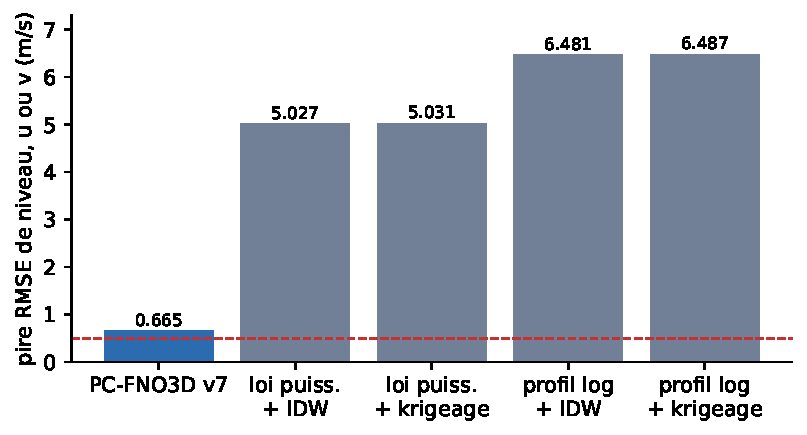
\includegraphics[width=0.85\linewidth]{figures/references_m8.pdf}
  \caption{Pire RMSE de niveau : PC-FNO3D contre les méthodes de référence (test synoptique).}
  \label{fig:references}
\end{figure}

L'erreur maximale de PC-FNO3D est 7,5 à 9,8 fois plus faible, et son $R^2$ minimal (0,991) est
loin devant celui des références (0,16 à 0,57). Trois études complémentaires du réseau ont été
menées :
\begin{itemize}
  \item \textbf{densité (E1)} : le modèle tient le DSO5 jusqu'à 50\,\% des capteurs ; aucune
        référence ne le tient, quelle que soit la densité ;
  \item \textbf{placement guidé par l'incertitude (E2)} : \textbf{résultat négatif} --- placer des
        capteurs là où l'incertitude est la plus forte fait pire que le hasard (2,39 contre
        1,28\ms) ;
  \item \textbf{capteur de secours (E3)} : sur ce réseau très dense, le krigeage (0,19\ms) remplace
        mieux un capteur en panne que la reconstruction 3D (1,50\ms).
\end{itemize}

\subsection{Fiabilité, alertes et éolien}
Pour la v7, la première lecture du DSO6 était non conforme (couverture de 75 à 81\,\%) ; une
seconde lecture, avec un facteur de calibration choisi sur la validation après ce premier verdict,
est conforme (87 à 91\,\%) mais n'est pas une mesure indépendante, et elle est publiée comme telle.
Le détecteur d'anomalies de capteurs (AN1) suit le même schéma : la v1 ne détectait que 5,2\,\% des
dérives ; la v2, fondée sur la cohérence avec les voisins et un modèle de site appris sur
l'entraînement, en détecte 100\,\% avec 2,2\,\% de fausses alertes (seconde lecture). Sur un parc
éolien de démonstration (3 éoliennes, 12\,MW), l'écart de production entre vent reconstruit et vent
vrai est de 1,71\,\% (seuil 5\,\%, EOL1).

\section{Domaine réel du Grand Tunis}

\subsection{Lignée des modèles}
\begin{figure}[H]
  \centering
  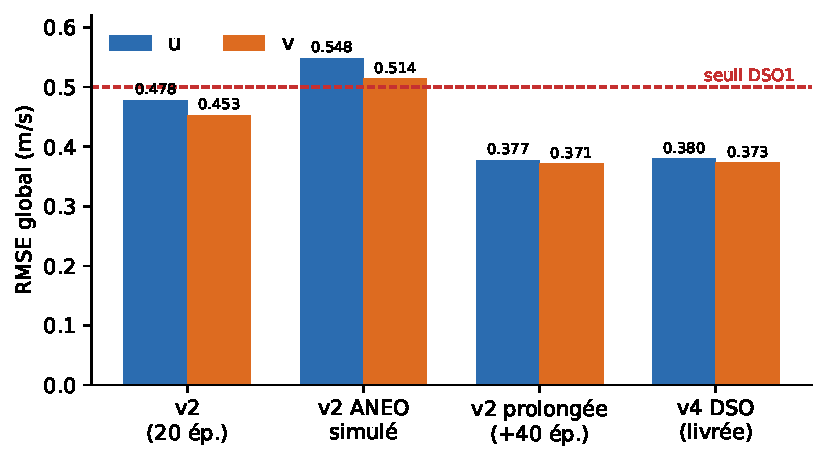
\includegraphics[width=0.85\linewidth]{figures/lignee_grand_tunis.pdf}
  \caption{RMSE global sur le test du Grand Tunis (180 instants) selon la version du modèle.}
  \label{fig:lignee}
\end{figure}

\begin{itemize}
  \item \textbf{v1} (champ entier, 25 canaux) : arrêtée à l'époque 14, $R^2$ de validation
        $u$ 0,78 / $v$ 0,73 ; le diagnostic montre que le profil ERA5 seul fait mieux (0,95 / 0,97) :
        il manque une entrée, ce n'est pas un défaut de code ;
  \item \textbf{v2} (34 canaux, correction d'ERA5, 20 époques) : $R^2$ de validation 0,986 / 0,992 ;
        test : RMSE global 0,478 / 0,453\ms, erreur de direction 3,9° ;
  \item \textbf{v2 ANEO simulé} (couche dense synthétique au lieu des stations) : moins bonne
        (0,548 / 0,514\ms) : une couche dense simulée n'apporte rien une fois le profil ERA5 en
        entrée ;
  \item \textbf{v2 prolongée} (+40 époques) : 0,377 / 0,371\ms, $R^2 \ge 0{,}98$ à tous les
        niveaux, erreur de direction 3,3° ; seul le niveau 25\,m reste au-dessus de 0,5\ms ;
  \item \textbf{v4} (affinage orienté DSO, $w$ par continuité) : livrée (section suivante).
\end{itemize}

\subsection{Décision de livraison de la v4}
La règle, écrite avant le test de la v4, était : la v4 n'est livrée que si elle n'est pas moins
bonne que la v2 prolongée sur DSO1, DSO4, DSO5 et les vraies mesures, avec une tolérance de 1\,\% et
aucune station dégradée de plus de 3\,\%. Le tableau~\ref{tab:v4} montre qu'elle l'est.

\begin{table}[H]
\centering
\caption{v4 (livrée) contre v2 prolongée, test du Grand Tunis (180 instants).}
\label{tab:v4}
\begin{tabularx}{\linewidth}{@{}Xccl@{}}
\toprule
Critère & v4 & v2 prolongée & Seuil\\
\midrule
RMSE global $u$ / $v$ (m/s) & 0,380 / 0,373 & 0,377 / 0,371 & ---\\
Pire RMSE de niveau (m/s) & 0,528 & 0,530 & $\le 0{,}5$\\
DSO2 ($w$ par continuité) & $1{,}05\cdot10^{-5}$ & $1{,}05\cdot10^{-5}$ & $\le 10^{-4}$\\
DSO4 (s) & 0,302 & 0,302 & $<1$\\
DSO5 25\,\% des entrées (m/s) & 0,535 & 0,537 & $\le 0{,}7$\\
Stations réelles, moyenne (m/s) & 2,469 & 2,467 & $\le$ v2 + 1\,\%\\
\bottomrule
\end{tabularx}
\end{table}

Sur la v4, le DSO6 est \textbf{conforme} dès la première lecture : couverture de l'intervalle à
80\,\% de 0,878 pour $u$, 0,883 pour $v$, 0,841 pour $w$ et 0,879 pour la vitesse, avec des
corrélations de Spearman positives (0,16 à 0,50) (figure~\ref{fig:dso6}).

\begin{figure}[H]
  \centering
  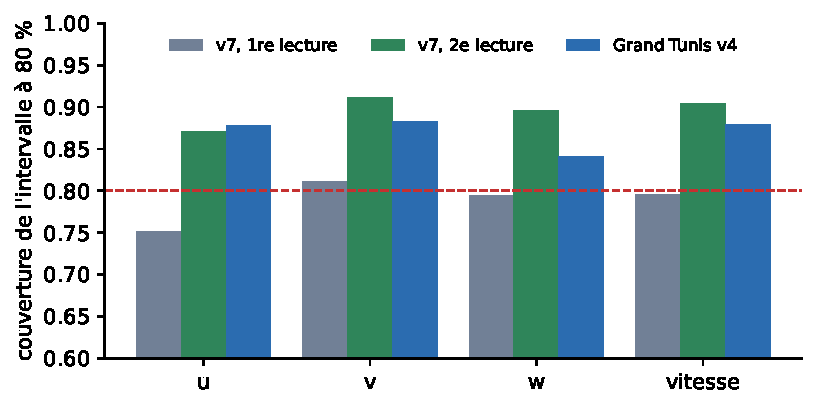
\includegraphics[width=0.82\linewidth]{figures/dso6_couverture.pdf}
  \caption{Couverture de l'intervalle à 80\,\% (DSO6).}
  \label{fig:dso6}
\end{figure}

\subsection{Validation sur les mesures réelles}
\begin{figure}[H]
  \centering
  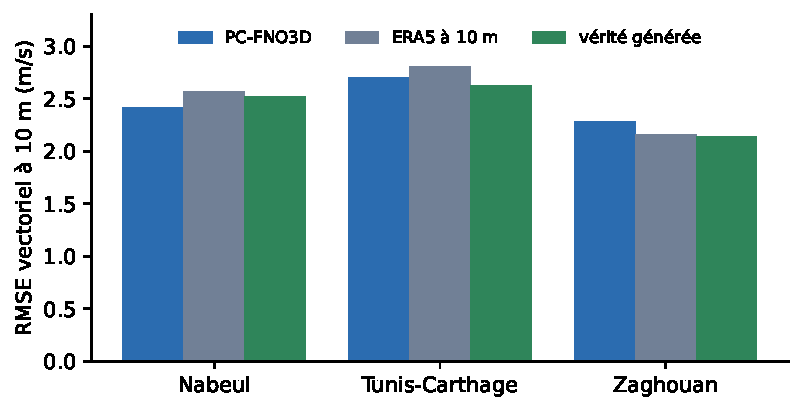
\includegraphics[width=0.82\linewidth]{figures/stations_reelles.pdf}
  \caption{Erreur aux stations réelles (station exclue de l'entrée), vent à 10\,m.}
  \label{fig:stations}
\end{figure}

Aux stations, le modèle est au niveau d'ERA5, un peu meilleur à Nabeul et Tunis-Carthage, un peu
moins bon à Zaghouan (figure~\ref{fig:stations}). Il reproduit la vérité générée, dont l'erreur
propre face aux stations est du même ordre : \emph{la limite est la vérité d'apprentissage, pas le
réseau}. Les erreurs de direction sont de 27 à 38° pour les trois sources, ce qui reflète la part
locale du vent qu'aucune n'explique. En altitude, sur les radiosondages de Tunis-Carthage (9 à 11
sondages par couche de 250\,m sur les blocs de test), le modèle fait mieux qu'ERA5 dans toutes les
couches de 0 à 1\,000\,m (RMSE vectoriel 1,95 à 2,34 contre 2,07 à 2,54\ms), avec un biais de
vitesse plus faible près du sol (0,58 contre 1,04\ms sous 250\,m).

\subsection{Affinage sur les stations : un gain illusoire}
La v3 a été affinée en prenant les trois stations comme cibles supplémentaires. Le modèle final
semblait spectaculaire à Tunis-Carthage et Zaghouan (figure~\ref{fig:v3}), mais moins bon à Nabeul,
où la station, abritée, mesure trop peu de vent. La \textbf{validation croisée spatiale}, où la
station jugée n'est jamais une cible, tranche : les gains tombent à $-1{,}5$, $-0{,}4$ et
$-0{,}5$\,\%, dans le bruit de mesure. La v3 a appris une \textbf{correction de site} aux points
cibles --- des taches de 0,8\ms dans le premier kilomètre autour des stations, moins de 0,1\ms au-delà
de 3\,km --- et non un meilleur champ entre les stations. La règle fixée à l'avance (gain moyen d'au
moins 5\,\% et d'au moins 3\,\% sur deux stations jamais vues) l'écarte, tout comme la variante v3b.

\begin{figure}[H]
  \centering
  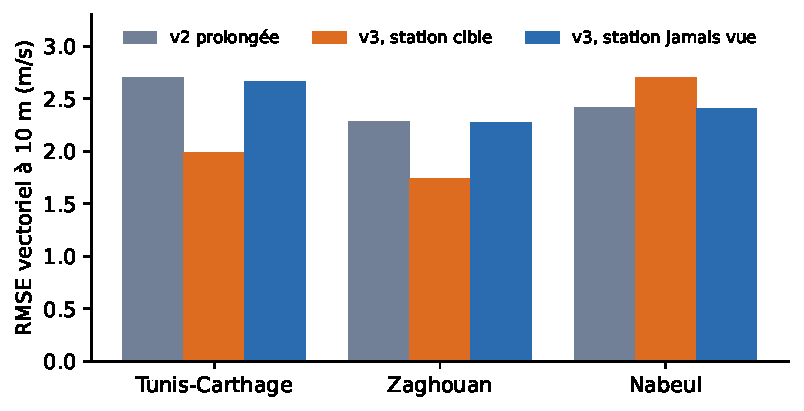
\includegraphics[width=0.82\linewidth]{figures/v3_validation_croisee.pdf}
  \caption{Affinage v3 : station cible contre station jamais vue (validation croisée spatiale).}
  \label{fig:v3}
\end{figure}

\section{Plan de déploiement du réseau ANEO (OS6)}
L'étude OS6 simule l'apport de capteurs ANEO : un capteur simulé est une maille où le modèle reçoit
la vérité de surface, comme une station réelle. 11\,890 emplacements candidats respectent les
contraintes (terre ferme, altitude au plus 650\,m, pente au plus 20°, 1\,km du bord et des autres
capteurs). Un placement glouton ajoute 5 capteurs par étape là où l'erreur résiduelle de validation
est la plus forte, jusqu'à 200 ; la courbe de dimensionnement compare ensuite, sur le test, le
placement optimisé, une grille régulière et des tirages au hasard (figure~\ref{fig:os6}).

\begin{figure}[H]
  \centering
  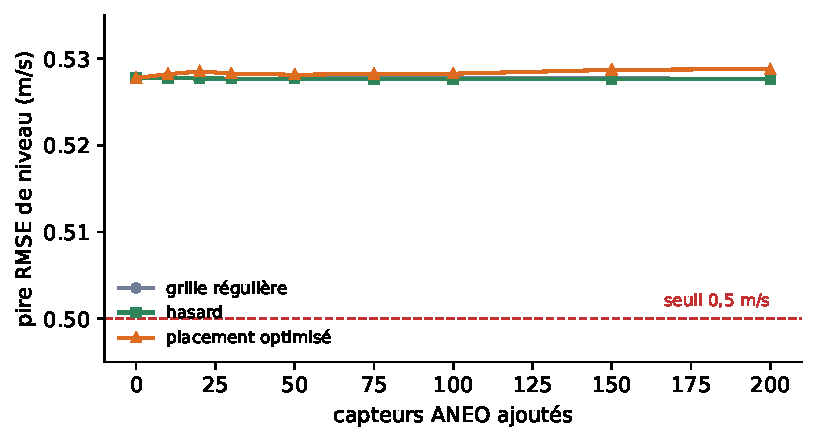
\includegraphics[width=0.82\linewidth]{figures/os6_courbe.pdf}
  \caption{OS6 : pire RMSE de niveau selon le nombre de capteurs ajoutés (test, 180 instants).}
  \label{fig:os6}
\end{figure}

Le résultat est \textbf{négatif} : de 10 à 200 capteurs, toutes les stratégies restent à
0,5326\ms de RMSE vectoriel et 0,528\ms au pire niveau, à $\pm0{,}0003$\ms près ; le placement
optimisé est même très légèrement moins bon. Aucun nombre de capteurs n'atteint le seuil (NET1 et
NET2 non conformes). Ce n'est pas un défaut de la simulation : les capteurs simulés reçoivent bien
la vraie valeur de surface. C'est une propriété du modèle livré : entraîné avec le treillis ERA5 et
trois stations, il s'appuie sur la grande échelle et traite une mesure ponctuelle comme une
correction locale. \textbf{Dimensionner le réseau demande un modèle entraîné à exploiter des
capteurs denses}, ce qui suppose un nouvel entraînement.

\section{Prévision à +24 et +48\,h (OS7)}
Le même modèle est nourri par la prévision GFS au lieu de la réanalyse. Les prévisions archivées
(NOAA, AWS) sont téléchargées pour chaque instant du cache aux échéances +24 et +48\,h (1\,000
échéances chacune), puis le modèle est affiné (v5) avec la même vérité et le même découpage, et
jugé sur 2022 contre GFS brut et la persistance (PREV1, PREV2), sur la décision de traitement de la
veille (PREV3) et sur les décisions agricoles aux stations (AGRI1, AGRI2).
\acompleter{Reporter ici les résultats d'OS7 (PREV1--3, AGRI1--2) une fois le calcul terminé.}

\section{Bilan de conformité}
Le bilan, produit automatiquement à partir des seuls résultats écrits, compte \textbf{18 critères
conformes, 4 non conformes, 1 proposé et 7 à mesurer} (tableau~\ref{tab:bilan}).

\begin{table}[H]
\centering
\caption{Bilan de conformité au cahier des charges (modèle livré v4).}
\label{tab:bilan}
\begin{tabularx}{\linewidth}{@{}lX@{}}
\toprule
Statut & Critères\\
\midrule
Conformes & DSO2, DSO4, DSO5, DSO6, REEL2, EOL2, DE1, DE2, DE3, PROD1, AN1 (seconde lecture), MCP1, API1, HIS1, EOL1 (parc de démonstration), REEL3, REEL4, NET2$^{*}$\\
Non conformes & DSO1 (0,528\ms au niveau 25\,m), DSO3 (0,805 : champ trop lisse), REEL1, NET1\\
Proposé & DSO7 (précision à densité réaliste, à fixer avec l'entreprise)\\
À mesurer & PREV1, PREV2, PREV3, AGRI1, AGRI2 (OS7), UX1, VIS1 (test utilisateur)\\
\bottomrule
\end{tabularx}
\par\smallskip\footnotesize $^{*}$ NET2 était compté conforme parce que la courbe existe ; la règle
corrigée exige aussi un nombre de capteurs suffisant, et NET2 est alors non conforme (5 non
conformes).
\end{table}

\section{Discussion}
Trois enseignements se dégagent.
\begin{enumerate}
  \item \textbf{La méthode fonctionne là où l'information existe} : sur le synthétique dense,
        PC-FNO3D surpasse largement les références et respecte la physique ; sur le réel, il
        améliore ERA5 en altitude et le vaut au sol.
  \item \textbf{La vérité d'apprentissage borne le résultat} : aux stations, le modèle ne peut pas
        faire mieux que le générateur qui lui sert de vérité ; les gains apparents d'un affinage
        sur les stations disparaissent dès qu'on juge sur des stations jamais vues.
  \item \textbf{Les règles fixées à l'avance ont évité trois fausses victoires} : la correction M1,
        l'affinage v3 et le placement guidé par l'incertitude auraient tous été retenus sur une
        lecture favorable du test.
\end{enumerate}

\chapter{Réalisation logicielle}
\label{chap:realisation}

\section{Architecture d'ensemble}
La figure~\ref{fig:systeme} présente la chaîne complète, des sources de données au navigateur de
l'utilisateur. Le calcul se fait là où sont le GPU et les poids (Google Colab), tandis que
l'adresse publique reste fixe grâce à un Worker Cloudflare et à un tunnel nommé.

\begin{figure}[H]
\centering
\begin{tikzpicture}[
  b/.style={draw, rounded corners=3pt, align=center, font=\footnotesize, minimum height=1.1cm,
            text width=3.3cm, fill=bleuespirt!8},
  s/.style={b, fill=gray!10},
  g/.style={b, fill=orange!12},
  fl/.style={-{Stealth[length=2mm]}, thick}]
  \node[b] (nav) at (0, 0) {Navigateur\\application ATOM Wind};
  \node[b] (worker) at (4.4, 0) {Worker Cloudflare\\atom.zelqane.com\\(clé injectée, cache)};
  \node[b] (tunnel) at (8.8, 0) {Tunnel Cloudflare\\nommé atom-origin};
  \node[s] (drive) at (0, -2.3) {Google Drive\\poids, cache, historique};
  \node[g] (modele) at (4.4, -2.3) {Modèle PC-FNO3D\\(GPU)};
  \node[g] (service) at (8.8, -2.3) {Service FastAPI\\et serveur MCP\\(Google Colab)};
  \node[s] (client) at (4.4, -4.6) {Clients de l'API\\et agents MCP};
  \node[s] (src) at (8.8, -4.6) {GFS (Open-Meteo),\\METAR, SYNOP};
  \draw[fl] (nav) -- (worker);
  \draw[fl] (worker) -- (tunnel);
  \draw[fl] (tunnel) -- (service);
  \draw[fl] (service) -- (modele);
  \draw[fl] (drive) -- (modele);
  \draw[fl] (src) -- (service);
  \draw[fl] (client) -- (service);
\end{tikzpicture}
\caption{Architecture de déploiement.}
\label{fig:systeme}
\end{figure}

\section{Le paquet \texttt{pcfno3d}}
Le notebook de recherche a été porté bloc par bloc en un paquet Python installable (41 modules,
environ 16\,800 lignes), qui est le seul chemin de code utilisé en production. Chaque bloc du
notebook devient un module ; la configuration et la géométrie sont passées explicitement au lieu
de variables globales (tableau~\ref{tab:modules}). Le portage a été validé en retrouvant
exactement la table de résultats du notebook.

\begin{table}[H]
\centering
\caption{Principaux modules du paquet.}
\label{tab:modules}
\begin{tabularx}{\linewidth}{@{}lX@{}}
\toprule
Module & Rôle\\
\midrule
\code{config}, \code{geometry} & Configuration typée ; grille, relief, masques, opérateurs discrets (gradient, résidu de masse)\\
\code{contract}, \code{cache} & Contrat de données ANEO ; tenseurs par instant et index\\
\code{dataset}, \code{features} & Entrée du modèle : canaux, vent géostrophique ajusté, entrée de production\\
\code{model}, \code{losses}, \code{train} & PC-FNO3D, perte physique, entraînement (EMA, OneCycle, reprise)\\
\code{evaluate}, \code{dso} & Métriques cumulées, verdicts DSO1 à DSO6\\
\code{inference}, \code{reliability} & Modèle de production, ensemble d'incertitude différé\\
\code{forcage}, \code{temps\_reel}, \code{gfs} & Forçage ERA5, temps réel GFS, archive GFS (OS7)\\
\code{alerts}, \code{windfarm}, \code{publish} & Alertes, post-traitement éolien, publication et exports NetCDF/CSV\\
\code{os6}, \code{atlas}, \code{baselines} & Plan du réseau, atlas éolien, méthodes de référence\\
\bottomrule
\end{tabularx}
\end{table}

Une interface en ligne de commande (\code{python -m pcfno3d <commande>}) expose toutes les étapes :
construction du cache, contrôle, entraînement, évaluation, reconstruction, alertes, publication,
service. Chaque commande accepte une configuration et des surcharges \code{--set section.clé=valeur}.

\section{Service web et sécurité}

\subsection{API REST}
Le service est une application FastAPI. Ses routes donnent la grille, les journées calculées, le
vent en un point et un profil vertical, la reconstruction à partir de mesures envoyées (fichier CSV
validé par le contrat), les exports NetCDF et CSV, la qualité du modèle servi, les alertes,
l'historique et les espaces métier (agriculture, production éolienne, maintenance, dimensionnement
de mât, espaces holding, chantier et environnement).

\subsection{Sécurité}
\begin{itemize}
  \item \textbf{fermé par défaut} : sans clé, toutes les routes répondent 401, sauf l'état de santé ;
  \item \textbf{clés d'API} de la forme \code{pcf\_<32 caractères>}, stockées uniquement par leur
        empreinte SHA-256, avec deux portées (lecture, administration), un quota par clé (réponse
        429) et un journal d'accès qui ne contient jamais de secret ; une révocation prend effet à la
        requête suivante ;
  \item \textbf{comptes utilisateurs} : mots de passe salés et dérivés par scrypt, blocage après
        cinq échecs, trois rôles (agriculteur, exploitant éolien validé par l'administrateur,
        administrateur) vérifiés côté serveur à chaque requête ;
  \item \textbf{secrets} : la clé du Worker n'est connue du service que par son empreinte, et les
        identifiants du tunnel ne transitent que par une variable d'environnement, jamais par le
        dépôt.
\end{itemize}

\subsection{Serveur MCP et assistant}
Le même modèle est exposé par un serveur MCP (\emph{Model Context Protocol}) de 22 outils :
consultation du vent et des profils, prévision en un point, décision agricole, fenêtres de
maintenance, valeur et influence des stations, simulation de panne, historique\dots{} Un agent
conversationnel peut ainsi lancer une simulation et en lire le résultat sans intervention (critère
MCP1). L'application intègre aussi un assistant fondé sur Claude, qui répond aux questions des
utilisateurs en appelant ces mêmes outils.

\section{Temps réel et prévision}
La réanalyse ERA5 arrive avec cinq jours de retard ; le temps réel utilise donc la prévision GFS
(via l'API Open-Meteo), calculée sur les mêmes mailles et avec les mêmes formules que le forçage
d'entraînement, et les mesures du jour : METAR de Tunis-Carthage et SYNOP de Zaghouan et Nabeul.
Le service calcule la journée en cours (heures passées avec les stations, heures futures en
prévision), le lendemain et le surlendemain, les garde en cache trente minutes et les archive sur
disque, ce qui permet de comparer plus tard une prévision au temps réel du même jour. Un ensemble
GEFS de 31 membres donne la probabilité de pouvoir traiter.

\section{L'application ATOM Wind}
L'application, construite à partir de la maquette fonctionnelle conçue pendant le projet, est une
page web sans étape de compilation, branchée sur l'API.

\begin{itemize}
  \item \textbf{Mon vent} : vent à 10\,m et à 2\,m, rafales, direction, pour un lieu choisi sur la
        carte, heure par heure ;
  \item \textbf{espace agriculteur} (application principale) : fenêtres de traitement et
        d'aspersion de J0 à J+2 avec la règle appliquée affichée, besoin en eau par la méthode
        FAO-56 \citep{allen1998} avec la température, l'humidité et le rayonnement de GFS ;
  \item \textbf{démonstration éolienne} : vent au moyeu et sur le rotor, production d'éoliennes de
        référence avec effets de sillage \citep{jensen1983}, rose des vents, carte du gisement et
        atlas annuel ;
  \item \textbf{vue 3D} : relief exagéré, lignes de courant, coupe horizontale, couleur selon la
        vitesse ou l'incertitude, colonnes de vent par nœud, relecture de la journée, fiche d'un
        point avec son profil et son intervalle à 80\,\% ;
  \item \textbf{tableau de bord} : indicateurs du service (stations actives, temps de
        reconstruction, résidu de masse de l'instant) et qualité du modèle servi ;
  \item \textbf{alertes} : station muette, résidu de masse hors seuil, vent fort, avec
        notifications par courriel, SMS ou WhatsApp ;
  \item \textbf{interface trilingue} français, arabe (de droite à gauche) et anglais ;
  \item \textbf{continuité de service} : quand le service est arrêté, le Worker sert le dernier
        état réel connu, signalé comme tel.
\end{itemize}

\acompleter{Insérer ici 3 à 5 captures d'écran de l'application (Mon vent, espace agriculteur,
vue 3D, tableau de bord) : déposer les images dans figures/ et utiliser \textbackslash includegraphics.}

\section{Qualité logicielle}
\begin{itemize}
  \item \textbf{tests} : 435 fonctions de test dans 42 fichiers, exécutées sur CPU en quelques
        minutes sur un mini-jeu de données synthétisé au format exact du générateur ; elles
        couvrent la physique (résidu de masse, continuité), l'API (sécurité, quotas), le contrat de
        données, la publication (atomicité face à un serveur simulé avec coupures), l'interface
        (dictionnaires de traduction) et le service Colab ;
  \item \textbf{reproductibilité} : même entrée et même version donnent la même sortie au bit près
        sur CPU ; sur GPU, l'écart reste de quelques $10^{-3}$\ms (calcul en bfloat16) ;
  \item \textbf{traçabilité} : chaque export porte l'empreinte des poids, des statistiques de
        normalisation et l'horodatage ; le cache porte un manifeste vérifiable ;
  \item \textbf{documentation} : fiches du modèle et des données, document d'intégration pour les
        équipes qui consomment la sortie, diagrammes UML.
\end{itemize}

\chapter*{Conclusion générale et perspectives}
\addcontentsline{toc}{chapter}{Conclusion générale et perspectives}
\markboth{Conclusion générale et perspectives}{}

Ce projet avait pour but de connaître le vent partout et à toutes les hauteurs utiles à partir de
mesures de surface éparses. Nous avons conçu, entraîné, évalué et mis en service PC-FNO3D, un
opérateur neuronal de Fourier tridimensionnel contraint par la physique.

\paragraph{Bilan.}
Sur le jeu synthétique, le modèle de référence reconstruit en 91\,ms un champ de 1,5 million de
nœuds, respecte la conservation de la masse ($2{,}6\cdot10^{-5}$), reste robuste avec un quart
des capteurs et divise par 7,5 à 9,8 l'erreur maximale des méthodes d'interpolation classiques.
Transposé au Grand Tunis, il apprend une correction du profil ERA5 : le modèle livré atteint une
erreur globale de 0,38\ms, garantit la conservation de la masse par construction, fournit une
incertitude calibrée (88\,\% de couverture pour l'intervalle à 80\,\%), fait mieux qu'ERA5 sur les
radiosondages et le vaut aux stations au sol. Il est servi par une API sécurisée, un serveur MCP
et l'application trilingue ATOM Wind, avec le temps réel et la prévision à trois jours.

\paragraph{Limites.}
Le niveau le plus bas (25\,m) reste à 0,53\ms, au-dessus du seuil ; le champ réel est un peu trop
lisse (rugosité 0,805) ; aux stations, la qualité est bornée par la vérité générée. L'étude OS6 a
montré que le modèle livré ne tire aucun gain de capteurs ajoutés, ce qui empêche de dimensionner
le réseau avec lui. Ces limites sont mesurées et documentées.

\paragraph{Apports personnels.}
\acompleter{Compétences acquises : apprentissage profond scientifique, physique de l'atmosphère,
ingénierie des données météorologiques, MLOps sur GPU distant, développement web et API, conduite
d'expériences avec règles de décision pré-enregistrées.}

\paragraph{Perspectives.}
\begin{itemize}
  \item \textbf{un modèle sensible aux capteurs} : réentraîner avec des capteurs simulés denses et
        tirés au hasard à partir de la vérité de surface, pour que le modèle exploite les mesures
        ANEO, puis refaire l'étude OS6 ;
  \item \textbf{la prévision OS7} : terminer l'affinage sur GFS et le juger contre GFS brut et la
        persistance ;
  \item \textbf{les données ANEO réelles} : brancher les premiers mâts Porteur et recaler le plan
        du réseau sur leurs mesures ;
  \item \textbf{l'état atmosphérique complet} : reconstruire aussi la température, l'humidité et la
        pression, déjà présentes en entrée ;
  \item \textbf{l'hébergement} : un service permanent au lieu d'une session GPU à la demande, et le
        test utilisateur prévu (UX1, VIS1) avec cinq personnes non spécialistes.
\end{itemize}


% ---------------------------------------------------------------- références et annexes
\cleardoublepage
\phantomsection
\addcontentsline{toc}{chapter}{Bibliographie}
\bibliographystyle{plainnat}
\bibliography{references}

\appendix
\chapter{Configuration et commandes}
\label{ann:config}

\section{Configuration du modèle livré (v4)}
Extrait du fichier \code{configs/grand\_tunis\_v4\_dso\_colab.yaml} (chemins omis).

\begin{lstlisting}
name: grand_tunis_v4_dso
model:                      # architecture v7 : les poids v7 servent de depart
  width: 48
  modes: [6, 32, 32]
  n_layers: 4
  pad: [4, 8, 8]
  proj_hidden: 128
  local_conv: true
  residuel_era5: true       # u, v = ERA5 au noeud + correction apprise
train:
  epochs: 15
  steps_per_epoch: 200
  batch_size: 1
  accum_steps: 2
  lr: 5.0e-5                # affinage depuis la v2 prolongee
  weight_decay: 1.0e-4
  ema_decay: 0.999
  grad_clip: 1.0
  select_by: dso            # pire rapport mesure / seuil des DSO (validation)
loss:
  lambda_mass: 5.0
  mass_ref: 5.0e-7
  lambda_bc: 0.1
  lambda_grad: 0.5
  w_weight: 2.0
mask:
  entree: era5_stations     # ERA5 10 m tous les 2,5 km + anemometres reels
  pas_era5_m: 2500.0
  p_station: 0.8
dso:
  rmse: 0.5
  r2: 0.95
  mass_rms: 1.0e-4
  roughness_range: [0.9, 1.1]
  time_s: 1.0
  rmse_25pct: 0.7
  min_level_cover: 0.05
\end{lstlisting}

\section{Principales commandes}
\begin{lstlisting}
python -m pcfno3d info                 # configuration effective et artefacts presents
python -m pcfno3d build-cache          # CSV journaliers -> tenseurs par instant
python -m pcfno3d check                # geometrie et verite
python -m pcfno3d validate f.csv       # contrat de donnees ANEO
python -m pcfno3d train                # reprend automatiquement
python -m pcfno3d evaluate             # metriques de test et verdicts DSO
python -m pcfno3d reconstruct --stem 004_120000 --altitude 120
pcfno3d apikey create app-web --scope read
pcfno3d serve --port 8000              # application, API (/api/docs), MCP (/mcp)
\end{lstlisting}

\section{Conventions}
\begin{itemize}
  \item $u$ positif vers l'est, $v$ vers le nord, $w$ vers le haut, en m/s ;
  \item direction météorologique (d'où vient le vent) : $(270^\circ - \operatorname{atan2}(v, u))
        \bmod 360^\circ$ ;
  \item altitudes des niveaux au-dessus du niveau de la mer ; hauteur au-dessus du sol fournie à
        part ;
  \item valeur absente : \code{NaN} dans les volumes reconstruits, $-9999$ dans les exports web.
\end{itemize}


\end{document}
